\section{Reihenschlussgenerator}
Bei diesem Generatortyp wird die Erregerwicklung in Serie mit der Ankerwicklung geschaltet. Da nun der Ankerstrom (=Erregerstrom) durch die Erregerwicklung ($D1$-$D2$) fließt, muss die Wicklung für deutlich höhere Ströme ausgelegt sein (wenige Windungen mit entsprechend größerem Querschnitt als bei der Fremd- oder Nebenschlusswicklung). Auch hier ist wieder auf den korrekten Stromfluss durch die Wicklung bei der Verschaltung zu achten, da die Maschine ansonsten ihren vorhandenen Remanenzfuss $\Phi_R$ durch die . Die Schaltung für den Reihenschlussgenerator ist in Abbildung \ref{abb:reihen_BKL_Messschaltung} dargestellt. 
\subsection{Bremsversuch}
\begin{figure} [htb]
    \centering
    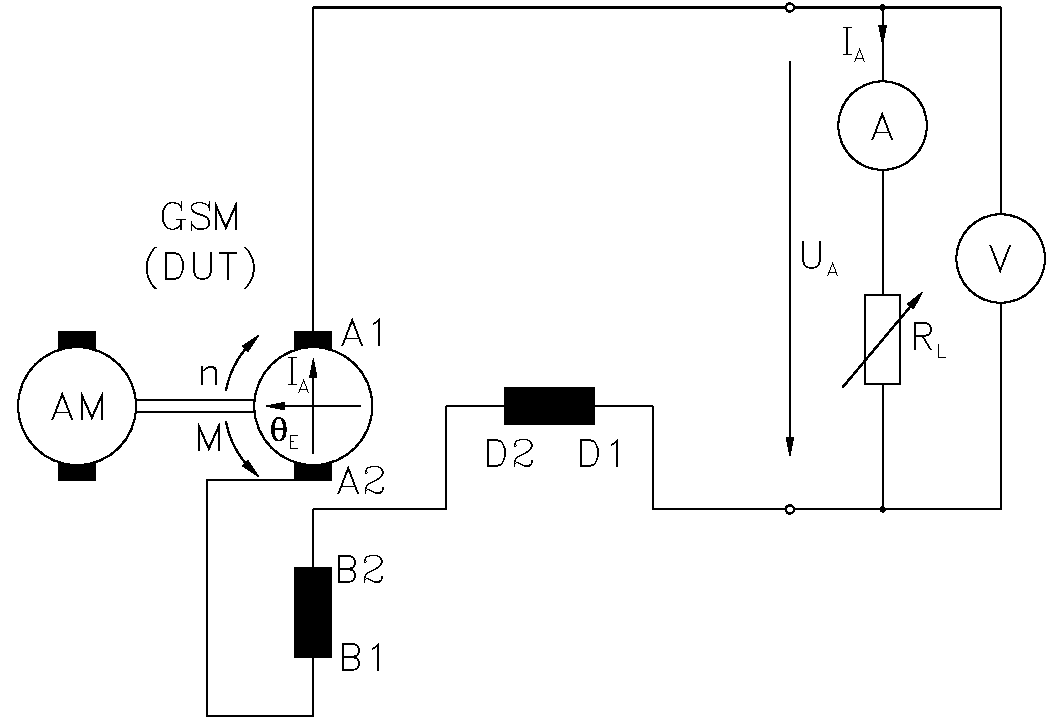
\includegraphics[width=0.55\textwidth, angle=0]{\currfiledir images/Bremskennlinie_reihenerregt}
    \caption{Messschaltung zur Durchführung eines Bremsversuchs des Reihen\-schluss\-gleich\-strom\-generators (GSM).}
    \label{abb:reihen_BKL_Messschaltung}
\end{figure}
Die erste Messung ist die äußere Kennlinie der Maschine, also der Verlauf der Ankerspannung in Abhängigkeit des Ankerstroms. Die Drehzahl wurde auf die negative Nenndrehzahl  ($n=n_N$) eingestellt. Die Belastung wurde über den Widerstand $R_L$ festgelegt, wodurch der Ankerstrom variiert wurde. Die so entstandene Kennlinie ist in Abbildung \ref{abb:reihenschluss_aussen} zu sehen.
\subsection{Innere Kennlinie}
Um die innere Kennlinie der Reihenschlussmaschine zu berechnen, wird die Äußere Kennlinie mit der folgenden Formel umgerechnet.
\begin{equation*}
    U_i=U_A + (R_A+R_D) I_A
\end{equation*}
Die Widerstandswerte können dem Maschinendatenblatt entnommen werden und entsprechen $R_A = \SI{0.78}{\ohm}$ und $R_D = \SI{0.1}{\ohm}$. Der Verlauf der Kennlinie ist ebenfalls in Abbildung \ref{abb:reihenschluss_aussen} dargestellt.
\input{\currfiledir Reihenschluss}
%\input{\currfiledir schaltung}